\section{Problem and Solution}
In this section we will lay out the problematic we wanted to adress during this project. Our chosen solution will be introduced and described.
\subsection{Problem}
The first part of the project was to define what are the needs of the elderly and their families in term of connectivity.

More and more people are connected to social networks and use internet to communicate. They share pictures or videos, send messages with their smartphones, tablet or PC. A lot of people who followed these new technilogies use it everyday with friends or family. A big part of the population is excluded as they are not able to use these new technologies. The goal is not to teach the old people how to use a computer or a smartphone but to have a device that would let them keep connected and included in the numerical world.

Especially in occidental countries, when the elderly are not able to take care of themself, they are going to an old people's home. Most of them would prefer to stay home longer. A device that would keep the old people connected with their family, check if everything is alright, make health tests could let the old people stay longer at their place.
\subsubsection{Younger generation needs}
To determine what are the young people needs, a quiz(survey) was put on internet to ask how young people would like to discuss with their grand parents.
The quiz contained questions of the type:
\begin{itemize}
\item{How often do you discuss with your grand parents?}
\item{What is the best way to do it? Social network, phone call, sms, visit them…}
\item{...}
\end{itemize}

Most of them wanted to have more contacts with their elders but not through available social networks (facebook, twitter, instagram, google+). This was mainly
due to the elderly beeing unfamiliar with these means of communication.
They mainly wanted to be able to share text and photos. Some of them would have liked to be able to make video calls.
\subsubsection{Elderly needs}
To define the needs of the elderly, a visit in an old peoples home (EMS) was organised and some questions about what they want and what they are able to do were asked to them and also some technical questions were asked to the nurses.

The general feeling is that the elderly generation is left out of the new technological world and developpment rarely take their input into consideration.

The questions to the nurses were more about the facilities old people have with new technologies. The results that came out of the discussion was that the old people don’t ear well sounds and are not able to define where the song is coming so putting an alarm on the device wouldn’t be a good idea. The interface has to be as simple as possible because they are lost if there are too many options. The device has to be big enough and shouldn’t break after a shock. The text on the device has to be big enough to be read by old people.

\subsection{Solution}
\label{chap: solution}
As the majority of the content people wanted to send to each other was text and images, the device at least needs a screen and some kind of user interface.
The challenge and purpose of the project was to find a user interface adapted to the elderly. The younger generation could use the internet on any device already available.
Different solutions were imagined. A device that connects to the TV with HDMI and display pictures, messages and videos on it.

A device that connects to the web with a 3G chip (don’t need the wifi and is more portable) or a device that contains only a wifi chip.

A device with a touch screen or only a screen. With physical buttons or not.

From the visit to the EMS we found out that:
\begin{itemize}
  \item{it was best if the device was portable. }
  \item{ A 7 inch screen was big enough }
  \item{ A flat device such as existing tablets was not suitable as it could get easily lost under things and the grip was not easy.}
  \item{ The color of the object is important as elderly tend to have many things and the device should be easily localisable}
  \item{ Sound was not a good medium to emit notification, visual stimulis was better.}
\end{itemize}


From these elements we decided to build a portable communication device dedicated to the elderly. This device has a 7 inch touchscreen has wifi and bluetooth
capabiities a battery and a no contact charging station. In parallel to this device a website and an app dedicated to the families of the elderly are linked to the device.

The families have an account wich is linked to a or several individual devices. The website and the app then allow the families to send photos and/or text directly to the connected device(s).
As soon as the device receives a new message a small LED starts to blink. When the elderly person opens the new message simply by touching the screen this triggers and automatic acknowledgment message to the sender.

The website also allows to adjust certain settings of the device such as screen brightness, in which order are the messages displayed, or the size of the text of the messages. The goal is to have the younger generation deal with all the setting up which might need a little more technological knowledge. The elderly can then relax and not think about anything outside the main purpose of the device.

\subsection{Vesta tab}

\begin{figure}[!htb]
    \centering
    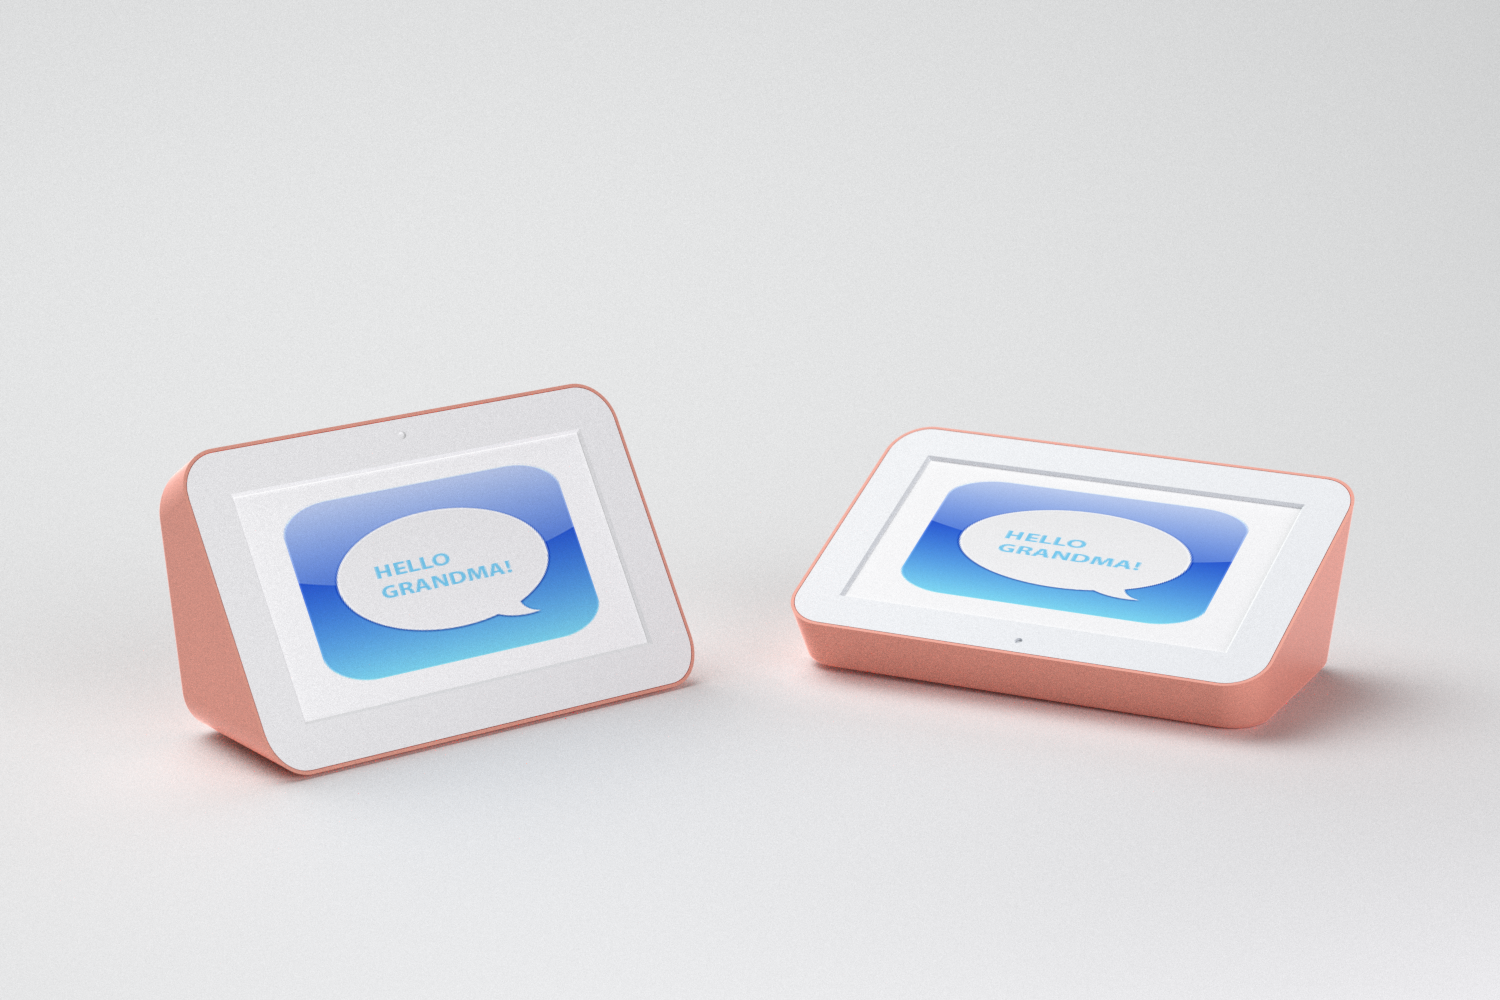
\includegraphics[width=0.9\textwidth,keepaspectratio]{chap/designFig/VisioRender5.png}
    \caption{Vesta tablet}
    \label{fig:vesta tablet}
\end{figure}

The Vesta tab is a tablet oriented towards the elderly. It has a capacitive touch screen, a wifi and bluetooth connection and a unique casing. The main usage at the moment is receiving and displaying pictures and text sent by the younger family via the dedicated website. As soon as a new image or text is received an LED blinks to inform the user of new content. The interface is designed to be very user friendly and easy to use.
